\section{Optimal Control of Unit Mass}

For each interval \(i-1<t\le i\), the force is constant:
\[
f(t)=x_i
\]
With unit mass, \(p''(t)=f(t)\). Over one unit interval,
\[
\dot p_i=\dot p_{i-1}+x_i,
\qquad
p_i=p_{i-1}+\dot p_{i-1}+\frac{1}{2}x_i
\]
Thus, for an integer time \(k\),
\[
\dot p(k)=\dot p(0)+\sum_{j=1}^k x_j
\]
and
\[
p(k)=p(0)+k\dot p(0)+\sum_{j=1}^k \left(k-j+\frac{1}{2}\right)x_j
\]

\textbf{(a)}
Here \(p(0)=\dot p(0)=0\). The objective is
\[
\int_0^{10} f(t)^2\,dt=\sum_{i=1}^{10}x_i^2=\|x\|_2^2
\]
The constraints \(p(10)=1\), \(\dot p(10)=0\), and \(p(5)=0\) can be written as
\[
Cx=d
\]
where the rows of \(C\) are the coefficient rows for \(p(10)\), \(\dot p(10)\), and \(p(5)\), which are linearly independent, so $C$ has full rank and $CC^T$ is invertible. Therefore the minimum-energy force vector is the minimum-norm solution
\[
x^\star=C^T(CC^T)^{-1}d
\]
% The result is
% \[
% x^\star=
% \begin{bmatrix}
% -0.045455\\
% -0.007576\\
% 0.030303\\
% 0.068182\\
% 0.106061\\
% 0.093939\\
% 0.031818\\
% -0.030303\\
% -0.092424\\
% -0.154545
% \end{bmatrix}
% \]
% The constraint check is
% \[
% \begin{bmatrix}
% p(10)\\ \dot p(10)\\ p(5)
% \end{bmatrix}
% =
% \begin{bmatrix}
% 1\\0\\0
% \end{bmatrix}
% \]
% and the energy is
% \[
% \sum_{i=1}^{10}x_i^2=0.062121
% \]

\begin{figure}[H]
    \centering
    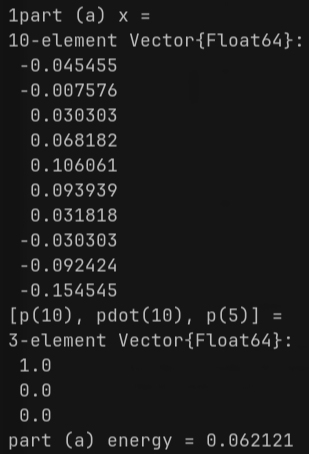
\includegraphics[width=0.3\textwidth]{img/4a.png}
\end{figure}

\begin{figure}[H]
    \centering
    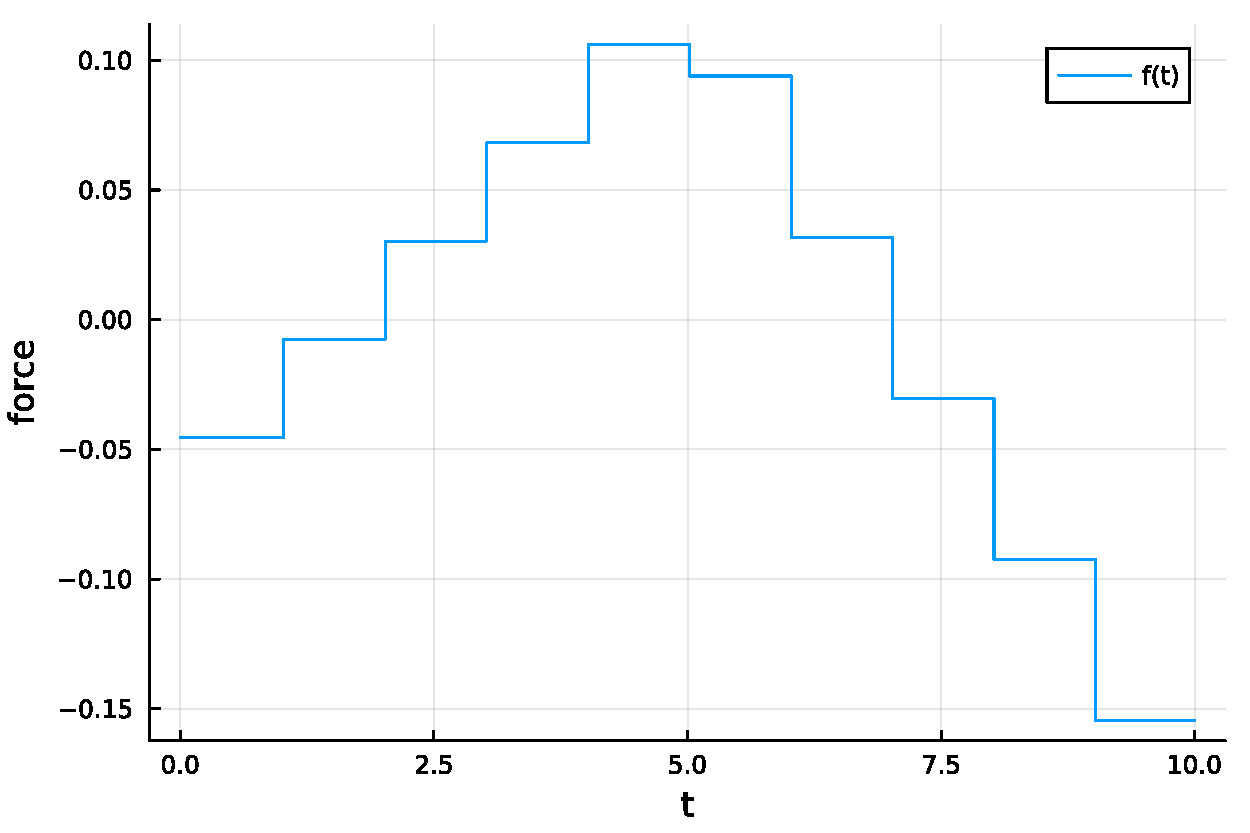
\includegraphics[width=0.82\textwidth]{img/p4a_force.pdf}
    \caption{Optimal piecewise-constant force for part (a)}
\end{figure}

\begin{figure}[H]
    \centering
    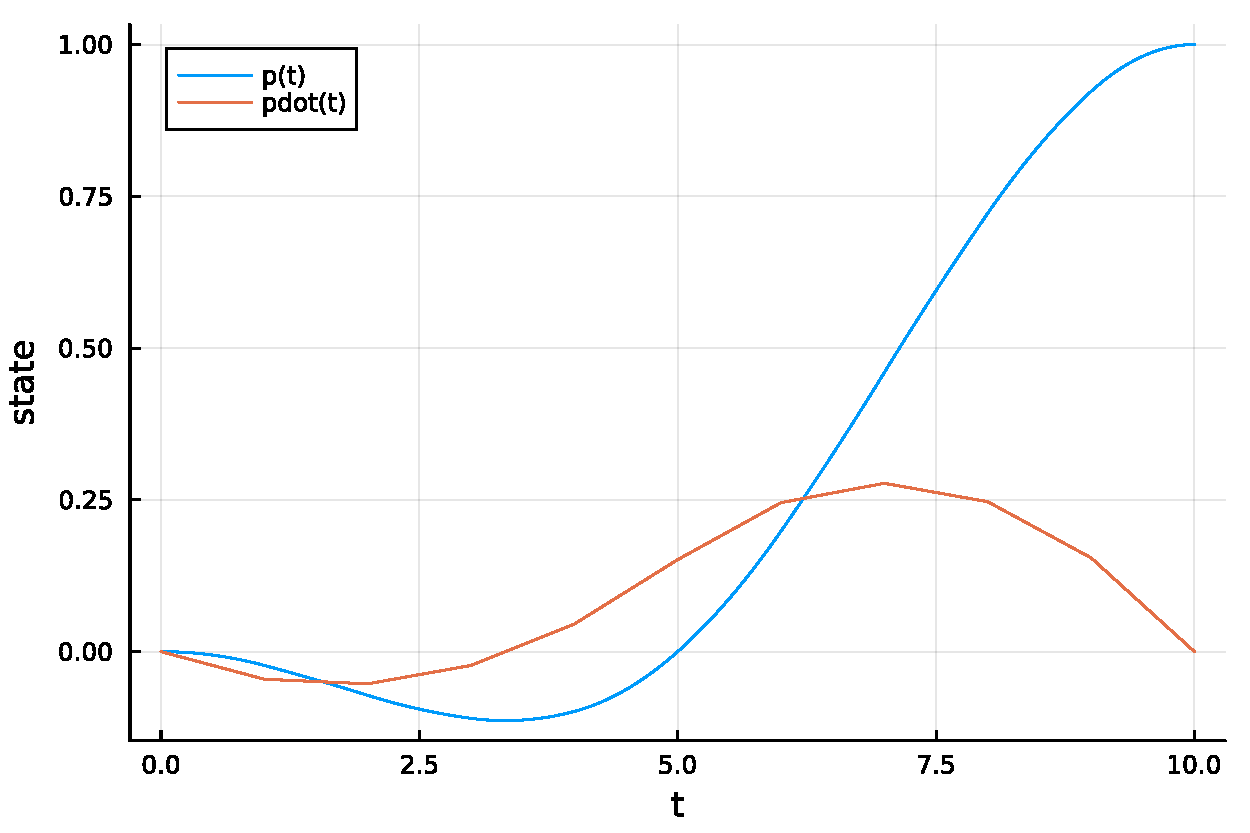
\includegraphics[width=0.82\textwidth]{img/p4a_state.pdf}
    \caption{Position and velocity produced by the optimal force}
\end{figure}

The force first keeps the mass near the origin so that the midpoint constraint \(p(5)=0\) is met, and then it pushes the mass toward \(p(10)=1\). Near the end it applies negative force to bring the velocity back to zero.

\textbf{(b)}
Now \(p(0)=0\) and \(\dot p(0)=1\). Let
\[
z=
\begin{bmatrix}
p(10)\\ \dot p(10)
\end{bmatrix}
=Bx+b
\]
where \(b=[10\;1]^T\) is the terminal state with zero force. Then
\[
J_1=\|Bx+b\|_2^2,
\qquad
J_2=\|x\|_2^2
\]
For each \(\mu>0\), I minimize
\[
J_1+\mu J_2
=
\|Bx+b\|_2^2+\mu\|x\|_2^2
\]
which gives
\[
x_\mu=-(B^TB+\mu I)^{-1}B^Tb
\]
% The endpoint with \(J_1=0\) is obtained by choosing the minimum-norm force that brings the mass exactly to the origin at rest. Numerically,
% \[
% J_1=1.97215\times 10^{-31}\approx 0,
% \qquad
% J_2=0.403030
% \]
% The endpoint with \(J_2=0\) is obtained by using no force, \(x=0\). Then
% \[
% J_1=10^2+1^2=101,
% \qquad
% J_2=0
% \]
Endpoints:
\begin{figure}[H]
    \centering
    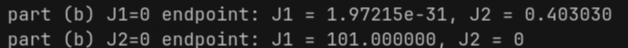
\includegraphics[width=0.6\textwidth]{img/4b.png}
\end{figure}

\begin{figure}[H]
    \centering
    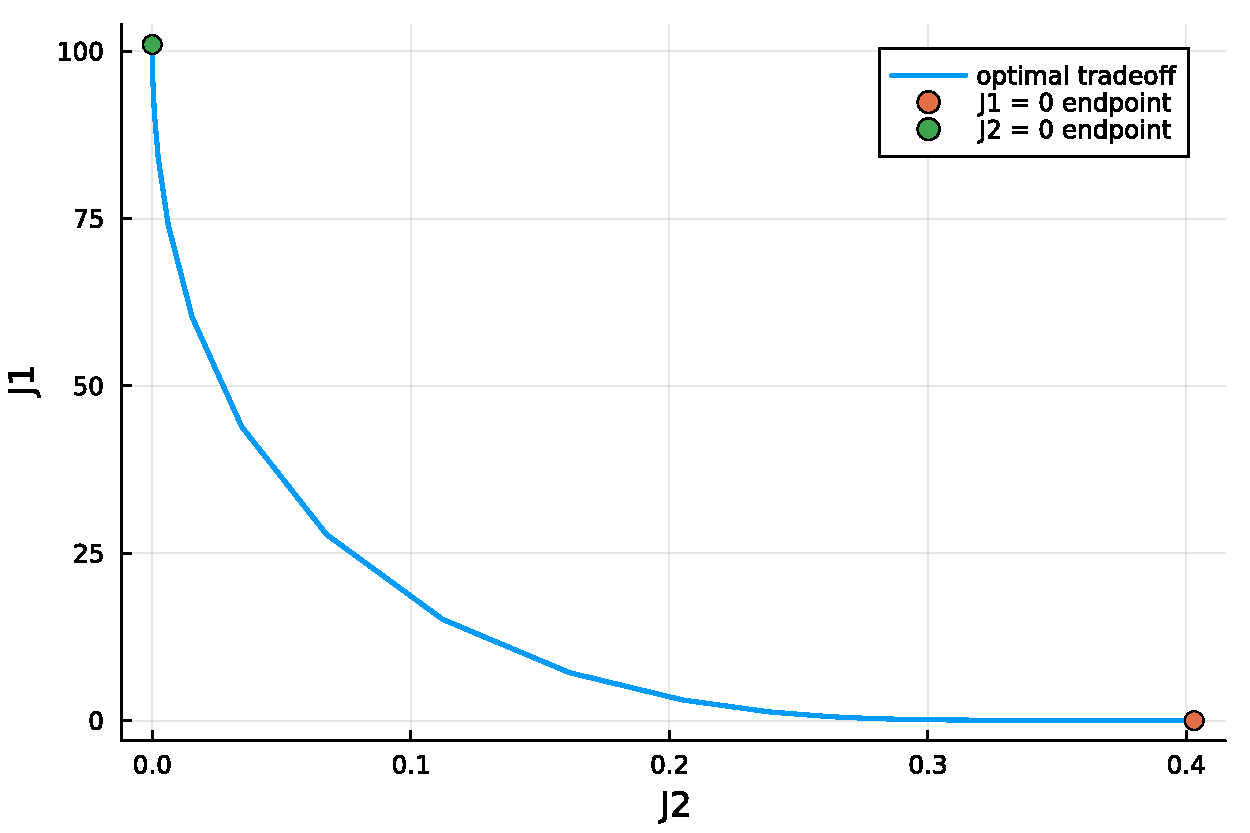
\includegraphics[width=0.82\textwidth]{img/p4b_tradeoff.pdf}
    \caption{Optimal trade-off between terminal error \(J_1\) and force energy \(J_2\)}
\end{figure}

\subsection{Code}
\begin{lstlisting}[language={}]
using LinearAlgebra
using Plots

p10 = [10 - j + 0.5 for j in 1:10]
v10 = ones(10)
p5 = [j <= 5 ? 5 - j + 0.5 : 0.0 for j in 1:10]

C = [p10'; v10'; p5']
d = [1.0, 0.0, 0.0]
x_a = C' * inv(C * C') * d

B = [p10'; v10']
b = [10.0, 1.0]
mu_values = 10.0 .^ range(-6, 6, length=50)
x_mu = [-(B' * B + mu * I) \ (B' * b) for mu in mu_values]
J1 = [norm(B * x + b)^2 for x in x_mu]
J2 = [sum(x.^2) for x in x_mu]
\end{lstlisting}
